\documentclass{article}
\title{Blockchain Technology SoS Reading Project}

\author{Pagoti Hemanth Naidu - 210050117 \\
Mentor: Shikhar Agrawal}
\date{may 2023}
\usepackage{xcolor}
\usepackage{graphicx}
\usepackage{adjustbox}
\usepackage{titlesec}
\usepackage{listings}
\usepackage{tikz}
\usepackage{amsmath}
\usepackage{hyperref}
\usepackage{tocloft}
\usepackage{tikz}
\usetikzlibrary{positioning}
\usetikzlibrary{shapes,arrows,calc,arrows.meta}
\usepackage{amsmath,bm,times}
\newcommand{\mx}[1]{\mathbf{\bm{#1}}} % Matrix command
\newcommand{\vc}[1]{\mathbf{\bm{#1}}} % Vector command
\renewcommand{\cftsecleader}{\cftdotfill{\cftdotsep}} % Add dots between section title and page number
\begin{document}
\tikzstyle{sensor}=[draw, fill=blue!20, text width=5em, 
text centered, minimum height=2.5em]
\tikzstyle{ann} = [above, text width=6em]
\tikzstyle{naveqs} = [sensor, text width=6em, fill=red!20, 
minimum height=12em, rounded corners]
\def\blockdist{2.3}
\def\edgedist{1}
\maketitle
\tableofcontents
\newpage
\section{Introduction}

Bitcoin was introduced in 2009 by Satoshi Nakamoto in response to the 2008 global financial crisis and the need for a decentralized, peer-to-peer electronic cash system. 
Nakamoto's vision was to create a currency free from central control, censorship-resistant, and capable of secure, borderless transactions.
\subsection{Demand \& Supply of Bitcoin}
Bitcoin's supply is regulated by Satoshi Nakamoto's algorithm, limiting the total number of bitcoins that can ever exist to 21 million.
The demand for bitcoin is determined by market forces and influenced by factors such as investor sentiment and adoption. 
Balancing supply and demand is essential for maintaining stability in the Bitcoin market and mitigating the risk of inflation.
\subsection{Double Spend Problem}
Satoshi Nakamoto's design of Bitcoin ensures that money can only be spent once through the concept of ownership and peer-to-peer networks. With public keys, everyone can know how much each owner possesses while maintaining anonymity. 
Hash functions are used for encoding transactions and mining purposes, while proof of work enables Bitcoin to function as a cryptocurrency. 
The tamper-proof nature of blockchain ensures that once transactions are added, they cannot be modified, and each block in the blockchain contains the hash of the previous block.
Smart contracts are self-executing contracts with the terms of the agreement directly written into code, automating and enforcing the agreed-upon conditions without the need for intermediaries. 
They enable secure and transparent transactions in various applications, from finance to supply chain management.
\section{Motivation}
\subsection{Blockchains in High Level}
\begin{itemize}
    \item Blockchain utilizes a tamperproof data structure that ensures data integrity and security.
    \item Starting with a genesis block, each subsequent block in the chain holds information in the form of bitstrings or binary representations.
    \item Once data is added to a block and appended to the chain, it becomes immutable and cannot be removed or altered.
    \item This feature of blockchain, along with its decentralized and distributed nature enables various applications such as cryptocurrency, smart contracts and trust.
\end{itemize}
\subsection{Applications}
\begin{itemize}
    \item \textbf{Governance}: Land records, health records, transportation data, virtual currency, electronic wills, passport, identification, etc.
    \item \textbf{Commercial}: supply chains, auctions, gaming, sale of music, financial services, smart grid etc.
    \item \textbf{Disruptive}: Cryptocurrencies, Initial Coin Offerings
\end{itemize}
\section{cryptocurrency}
Bitcoin has no central trudtrd authority, cryptography brings in trust and peer to peer networks provide decentralization. Bitcoin satisfies the characteristics of acceptability, portability, durability, divisibility, and fungibility.
\begin{itemize}
\item \textbf{Acceptability}: Bitcoin is widely accepted as a form of payment and store of value.
\item \textbf{Portability}: Bitcoin can be easily transferred and accessed across geographical boundaries.
\item \textbf{Durability}: Bitcoin's digital nature makes it resistant to physical damage or deterioration.
\item \textbf{Divisibility}: Bitcoin is divisible into small units, allowing for precise transactions of any value.
\item \textbf{Fungibility}: Bitcoin units are interchangeable, meaning that each unit holds the same value and can be exchanged without distinction.
\end{itemize}
Each transaction is brodcasted among all so that double spend is avoided. \\
Consensus protocols are mechanisms used in blockchain networks to achieve agreement among participants on the validity of transactions and the order in which they are added to the blockchain and this is also know as proof of work.
\section{Peer to Peer}
A permissionless, distributed system allows an arbitrary number of participants to join or leave at any time, enabling seamless peer-to-peer transactions where individuals have the freedom to pay anyone within the network, fostering inclusivity and decentralization.
\subsection{Consensus Protocol}
\begin{itemize}
\item To establish consensus in a protocol, cryptography is employed to secure transactions and validate the integrity of the data. 
\item While a peer-to-peer network enables direct communication and information sharing among participants. 
\item The proof-of-work mechanism adds a layer of computational effort to validate transactions and prevent malicious behavior, and Merkle trees provide an efficient and verifiable way to store and verify the integrity of large sets of data within the blockchain. 
\item Together, these components form the foundation for a robust and trustless consensus protocol.
\end{itemize}
\subsection{Popular P2P versions}
\subsubsection{Napster}
Napster was one of the earliest peer-to-peer networks that facilitated file sharing. It used a centralized server to maintain an index of available files, allowing users to search and download files directly from each other, enabling widespread file sharing but faced legal challenges due to copyright concerns.
\subsubsection{Gnutella}
Gnutella is a decentralized peer-to-peer network where participating nodes connect directly with each other. It operates on a query flooding mechanism, where search queries propagate across the network, and peers respond with matching files, ensuring a distributed and scalable file sharing system.
\subsubsection{Distributed Hash Table}
DHT is a decentralized peer-to-peer network architecture that provides efficient lookup and storage of key-value pairs. It operates by partitioning the hash space among participating nodes, enabling direct lookup and storage of data based on keys. DHTs provide fault tolerance, scalability, and efficient resource utilization in distributed systems and are commonly used in applications like BitTorrent and distributed storage systems.
\section{Hash functions}
Each block in the blockchain contains hash of the previous block, the hash is recognised as an unique ID.
\subsection{Basic properties of Hash functions}
\begin{itemize}
    \item Input to the hash function can be of any length.
    \item Output of the hash function should be of fixed size.
    \item Hah should be efficiently computed.
\end{itemize}
\subsection{Random Oracle}
It is like a black box that takes input and generates a random output based on that input. It provides a consistent and unpredictable response to any query. Random oracles are often used to model idealized cryptographic functions and serve as a building block for designing secure protocols and systems. \\
However, in practice, real-world hash functions are used as a substitute for random oracles.
\subsection{Properties of Cryptographic Hash functions}
\subsubsection{Collision Resistence}
Collision resistance, in the context of cryptographic hash functions, means that it is computationally infeasible to find two different inputs that produce the same hash output. It ensures that a small change in the input will result in a significantly different hash value, making it difficult to forge or manipulate data without detection. \\
The birthday paradox states that in a group of relatively few people, the probability of two individuals sharing the same birthday is surprisingly high.
\subsubsection{Hiding}
suppose r takes values from $r_1$, $r_2$, $r_3$, ....., $r_n$ with probability  $p(r_1)$, $p(r_2)$, $p(r_3)$, ....., $p(r_n)$. \\
The minimum entropy is defined as follows 
$$min-entropy = min_{i=1}^{n} -log(x_i)$$
where a secret value r is chosen from a probability distribution with high min-entropy and combined with another value x to compute the hash h(x\textbar\textbar r), it is infeasible to find the original value of x given only the hash h(x\textbar\textbar r). \\
\subsubsection{Puzzle Friendliness}
Hash function is puzzle friendly if for every N bit output Y if K is choosen from a probability distribution with high minimum entropy, then it is infeasible to find X such that 
$$H(K||X) = Y$$
in time significantly less than O($2^N$).
\subsection{Proof of Work}
\begin{itemize}
\item Miner selects pending transactions.
\item Miner combines hash of previous block, nonce, and transactions.
\item Nonce is of 16 bits, miner can include any number of transactions.
\item Miner adjusts nonce until the resulting block hash meets the threshold for network consensus, creating the next block.
\item Once a valid block is created it should be brodcasted to other miners for verification.
\end{itemize}
\section{SHA256 and Merkle Trees}
Here's a high-level overview of how SHA-256 works:
\begin{itemize}
\item \textbf{Padding}: The input message is padded with length of message to ensure it meets certain requirements for the SHA-256 algorithm. Padding includes adding bits to the message to make it a multiple of 512 bits.
\item \textbf{Initialization}: An Initialization Vector (IV) is a predetermined set of initial values used to initialize the compression process in certain compression algorithms, ensuring consistent and reproducible compression results for the same input data.
\item \textbf{Processing}: The padded message is divided into blocks of 512 bits, and the algorithm processes each block sequentially. The processing involves a series of logical and bitwise operations, including message expansion, data mixing, and bitwise operations such as AND, OR, and XOR.
\item \textbf{Compression}: Each block is compressed using a combination of logical and bitwise operations, updating the state of the hash values.
\item \textbf{Finalization}: Once all the blocks have been processed, the resulting hash value is obtained by concatenating the updated hash values.
\end{itemize}
Miners use Merkle trees (also known as Merkle hash trees) as an efficient and secure way to summarize a large set of transactions within a blockchain. These trees play a crucial role in the creation of the next block in the blockchain. Let's walk through the process:
\begin{itemize}
    \item Miners gather valid transactions and sort them. They hash each transaction individually and combine the hashed values in pairs until a single root hash, known as the Merkle root, remains at the top of the tree.
    \item The Merkle root is included in the block header along with other block information. Miners attempt to find a nonce value that, when hashed with the block header, produces a hash that is less than the threshold.
\end{itemize}
\subsection{Advantages of Merkle Trees}
\begin{itemize}
    \item Merkle trees enable efficient verification and tamper detection, making it difficult for a miner to modify a specific transaction without changing the Merkle root.
    \item If a miner want to add or Modify a transaction while solving the puzzle it can be done in O(log(M)) operations where M is no of transactions included.
    \item Light clients(New commer of Bitcoin) require fewer resources, enabling users with limited capabilities to participate in blockchain networks.
\end{itemize}
\subsection{Prooving to Light Client}
There is a situation that A is a light clinet and B need to proove that one of his transaction happend to C to A then B can provide A with a compact proof known as a Merkle proof. \\
This proof consists of the transaction, its corresponding Merkle path, and the Merkle root. A can then verify the validity of the transaction by using the Merkle proof to trace the transaction's inclusion in the Merkle tree and comparing the computed Merkle root with the one stored by A.
\subsection{Full Client using Merkle Trees}
If a full client want to discard any of the transaction he stored he can still proove that remaing transactions belonging to the same merkle tree which may not be happend if he stores in a naive way i.e concatenating all the transactions.
\section{Bitcoin Transactions}
\subsection{Block Header contents}
The block header in a blockchain typically contains the following elements:
\begin{itemize}
    \item \textbf{Previous Block Hash}: Hash of the preceding block in the blockchain.
    \item \textbf{Merkle Root}: Hash of all the transactions included in the block.
    \item \textbf{Timestamp}: The time when the block was created, which is used after to find appropriate threshold.
    \item \textbf{Nonce}: A number used in the mining process to find a valid block hash.
    \item \textbf{threshold}: 4 Bytes are used to represnt threshold also known as bits, to save space instead of storing 256 bits.
    $$bits = b_1b_2b_3b_4$$
    $$Threshold = b2_2b_3b_4 * 256^{b_1 - 3}$$
\end{itemize}
\subsection{Digital Signatures}
Digital Signatures are hard to forge, easy to create and easy to verify. \\
These signatures use the below three alogorithms to complete the need:
\subsubsection{Generation of shared, public key pair}
This uses GenerateKeys algorithm which takes key size as the parameter and generates a key pair in which shared key is kept secret and public key is known to everyone.
\subsubsection{sign the message}
This uses Sign algorithm which takes message and shared key as the algorithm and encypts the message, in this case message is typically a transaction. 
\subsubsection{verify the signature}
This uses Verify algorithm which takes the message, signature and cipher text and verify the signature, this is done by everyone to verify transactions.
\subsection{ECDSA}
Elliptic Curve Digital Signature Algorithm is a cryptographic algorithm used for generating and verifying digital signatures, in which public key is 512 bits, shared key is 256 bits, signature is 512 bits and the message should be 256 bits.\\
Hash the message using SHA256 as many of the messages are not of 256 bits.
\subsection{Transactions}
Assume A($SK_A,PK_A$) want to pay B($SK_B,PK_B$),  A has to make a transaction himself and sigh it with his shared key as discussed above. \\
Now the problem is how a miner verify this transaction is valid or not.
\subsubsection{Structure of bitcoin transactions}
\begin{center}
\begin{tikzpicture}[>={Latex[scale=1.5]}]
    %% Encoder
    \node (naveq) [naveqs] {Transaction};
    %% Inputs
    \draw[<-] ($(naveq.south west)!0.9!(naveq.north west)$) -- +(-\edgedist,0) node [left] {$(SK^{i}_0,PK^{i}_0)$};
    \draw[<-] ($(naveq.south west)!0.75!(naveq.north west)$) -- +(-\edgedist,0) node [left] {$(SK^{i}_1,PK^{i}_1)$};
    \draw[<-] ($(naveq.south west)!0.6!(naveq.north west)$) -- +(-\edgedist,0) node [left] {$(SK^{i}_2,PK^{i}_2)$};
    \draw[<-] ($(naveq.south west)!0.45!(naveq.north west)$) -- +(-\edgedist,0) node [left] {$(SK^{i}_3,PK^{i}_3)$};
    \draw[<-] ($(naveq.south west)!0.30!(naveq.north west)$) -- +(-\edgedist,0) node [left] {$(SK^{i}_4,PK^{i}_4)$};
    \draw[<-] ($(naveq.south west)!0.15!(naveq.north west)$) -- +(-\edgedist,0) node [left] {$(SK^{i}_5,PK^{i}_5)$};
    %% Outputs
    \draw[->] ($(naveq.south east)!0.9!(naveq.north east)$) -- +(\edgedist,0) node [right] {$(SK^{o}_0,PK^{o}_0)$};
    \draw[->] ($(naveq.south east)!0.75!(naveq.north east)$) -- +(\edgedist,0) node [right] {$(SK^{o}_1,PK^{o}_1)$};
    \draw[->] ($(naveq.south east)!0.6!(naveq.north east)$) -- +(\edgedist,0) node [right] {$(SK^{o}_2,PK^{o}_2)$};
    \draw[->] ($(naveq.south east)!0.45!(naveq.north east)$) -- +(\edgedist,0) node [right] {$(SK^{o}_3,PK^{o}_3)$};
    \draw[->] ($(naveq.south east)!0.3!(naveq.north east)$) -- +(\edgedist,0) node [right] {$(SK^{o}_4,PK^{o}_4)$};
    \draw[->] ($(naveq.south east)!0.15!(naveq.north east)$) -- +(\edgedist,0) node [right] {$(SK^{o}_5,PK^{o}_5)$};
  \end{tikzpicture}
\end{center}
Inputs are taken from earlier outputs of Bitcoin transactions, which consists hash of the transaction and index of the Block in which the transaction is present and some other feilds. Output pay Bitcoin to different public keys, each imput may correspond to multiple outputs. Reaming Bitcoin can be payed to himself by generating a new key pair, the transactions should be signed by shared keys of all inputs of the transaction.
\subsubsection{Transaction fee}
Transaction fees in Bitcoin are small amounts of Bitcoin paid by the sender of a transaction to incentivize miners to include and confirm the transaction on the network. The fee amount varies based on network congestion and transaction size. \\
If a sender wants to pay 1\% of his output as Transaction fee he decreases the output by 1\%. 
\subsubsection{Rules}
\begin{itemize}
    \item Output should not be negative in a transaction.
    \item sum of inputs must be greater than or equal to sum of outputs ina transaction.
    \item Whoever miner solves the puzzle can claim all the fee of the transcations he included and the mining fee.  
\end{itemize}
\subsubsection{Mining}
Miner selects some of the pending transactions, compute merkle root and djusts nonce until the resulting block hash meets the threshold for net-
work consensus, creating the next block.
\subsubsection{Coinbase transaction}
This the first transaction in which the miner claims the transaction fee and the mining reward, this transaction will not have any inputs it can create bitcoin i.e mining reward, which decreases exponentially so that no inflation occurs. Miner can claim his reward if he wins the game by creating next block.
\subsubsection{Double spend prevention}
There are set of rules which should be followed by miners so that double spend can be prevented these follows:
\begin{itemize}
    \item Any output of a transaction should be only spend once, such outputs are calles UTXO(Unspend Transaction Output).
    \item If any miner includes invalid transaction and succeeded in creating new block every other miner should discard that block, if the block is in some chain the chain is also discarded.
    \item When a miner creates a block with all valid transactions every other miner should delete the transaction which are in the new block from their respective transaction pool.
\end{itemize}
From the above miner can also change some arbitrary feilds in the coinbase transaction to complete the proof of work. \\
The length of block header is 80 bytes, satoshi managed to keep it small.
\section{Target Threshold}
If the threshold is set too small it takes miners so much time to complete the proof of work as it takes so many trails, if it is set too large then forks may appear insted of chain we will have trees. Target threshold should not be to large or small.  \\
Network delays while broadcasting block for verification should not be large because it may cause forks in the blockchain.
\subsection{Network propagation}
\begin{center}
    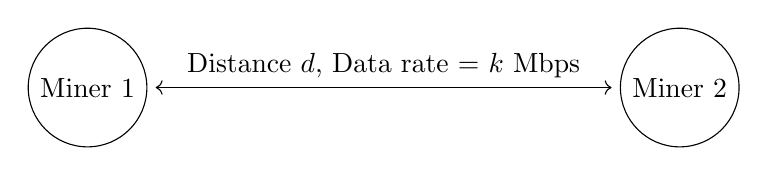
\begin{tikzpicture}
        % Define the nodes
        \node[draw, circle] (node1) {Miner 1};
        \node[draw, circle, right=6cm of node1] (node2) {Miner 2};
        
        % Draw the link
        \draw[<->, shorten >=3pt, shorten <=3pt] (node1) -- node[above] {Distance $d$, Data rate = $k$ Mbps} (node2);
    \end{tikzpicture}   
\end{center}
When miner 1 computes a block and want to transmit to miner 2 the delay is $\frac{d}{c}+\frac{b}{k}$, where b is the length of block size. Miner 2 verifies the block and broadcast it. \\
So the total time taken for end to end propagation of the block in peer to peer network is given below:
$$\sum_{i=1}^{n}\frac{d_i}{c}+\frac{b}{k_i}+p_i$$
where $p_i$ is the time taken for verification of the block, and the links are selected by the spanning tree algorithm for avoiding multiple transfers.
\subsection{How threshold is set}
Thers should be no situation like some miner solves proof of work while other miner broadcasting his bolck, it may lead to forks and double spend. So threshold is choosen such that each block takes 10 minutes to create. \\
The threshold cannot be constant becuase as the users of bitcoin increase the hashing power increases, so satoshi decided to update threshold every 2 weeks based on hashing power. Users use \textbf{A6} hardware for solving proof of work. This 2 weeks is defined in terms of no of blocks, in 2 weeks roughly 2016 blocks were created. \\
So threshold is updated after every 2016 blocks as follows:
$$threshold = threshold * \frac{T}{1209600}$$
T is Time taken for creation of prev 2016 blocks in sec, T can be found using timestamp in block header as follows:
$$T = timestamp(B_{2016n-1}) - timestamp(B_{2016(n-1)})$$
\subsection{Verification}
Ideally miner should follow \textbf{NTP} for the timestamp while solving proof of work.
\subsubsection{Rules for verification}
Miner accepts the recived block if:
$$t_k > median(t_{k-1},t_{k-2},t_{k-3}...... t_{k-11})$$
$$t_k < 2hours + Netwok adjust time$$
Nwtwok adjust time is defined as sum of miner local time according to NTP plus the median of the offsets with local times of his fellow peers.
\subsection{Deal with forks}
Satoshi's first rules were to slect longest chain if forks are present, if multiple longest chains were present should select the one with less timestamp.
\subsubsection{Chain weight}
If some attacker manages to create longest chain privately and broadcast afte he may kill the honest blocks to avoid this chain weight was used. \\
Chain weight uses the sum of expected work done for all the blocks
in the chain, if it is built using fake timestamps he may get caught.
expected work for creating i'th block is calculated as follows:
$$B_i = \lfloor \frac{2^{256}}{Threshold + 1} \rfloor$$
expected work for creating entire chain is calculated as follows:
$$\sum_{i=1}^{n}B_i$$
\section{Confirmation Time}
The confirmation time in blockchain refers to the amount of time it takes for a transaction to be validated and included in a block on the blockchain. The specific confirmation time can vary depending on the blockchain network and its consensus mechanism.\\
\textbf{Zero Confirmation}: A transaction that has been broadcasted but not yet added to a block or confirmed by the network.\\
\textbf{First Confirmation}: The first block in which a transaction is included, indicating its confirmation on the blockchain.\\
\textbf{Second Confirmation}: The second block in which a transaction is included, further validating its confirmation on the blockchain and increasing the level of confidence in its permanence.
\newpage
\begin{figure}
\centering
  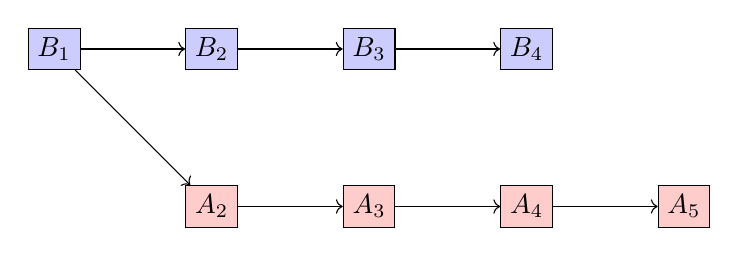
\begin{tikzpicture}[node distance=2cm, auto]
    % Nodes
    \node [draw, rectangle, fill=blue!20] (block1) {$B_1$};
    \node [draw, rectangle, fill=blue!20, right of=block1] (block2) {$B_2$};
    \node [draw, rectangle, fill=blue!20, right of=block2] (block3) {$B_3$};
    \node [draw, rectangle, fill=blue!20, right of=block3] (block4) {$B_4$};

    \node [draw, rectangle, fill=red!20, below of=block2] (a2) {$A_2$};
    \node [draw, rectangle, fill=red!20, right of=a2] (a3) {$A_3$};
    \node [draw, rectangle, fill=red!20, right of=a3] (a4) {$A_4$};
    \node [draw, rectangle, fill=red!20, right of=a4] (a5) {$A_5$};

    % Arrows
    \draw [->] (block1) -- (block2);
    \draw [->] (block2) -- (block3);
    \draw [->] (block3) -- (block4);
    \draw [->] (block1) -- (a2);
    \draw [->] (a2) -- (a3);
    \draw [->] (a3) -- (a4);
    \draw [->] (a4) -- (a5);
  \end{tikzpicture}
\end{figure}
\subsection{Double spend attack}
This attack was analysed by Satoshi himself, the above diagram shows the attack after $B_1$, so attacker creates another chain privately after $B_1$ to create double spend and kill the chain created by honest miners. \\
He creates until the other user confirms, i.e if the user waits till 3rd confirmation and attacker broadcast the transaction between $B_1$ and $B_2$, so the user checks if it is in $B_4$ are not, so attacker releases the chain after $A_5$ is created before $b_5$, otherwise he may not.
\begin{center}
\begin{tikzpicture}
    \coordinate (start) at (0,0); % Starting point
    \coordinate (end) at (6,0); % Ending point
    
    % Add height to the first and last coordinate
    \coordinate (p1) at (start |- 0,2);
    \coordinate (p2) at (end |- 0,2);
    
    \draw (p1) -- (start) -- (end) -- (p2); % Draw the line with added height
    
    \pgfmathsetmacro{\n}{5} % Number of divisions
    
    \foreach \i in {2,...,\n}{
        \pgfmathsetmacro{\x}{(\i-1)/\n*6} % Calculate the x-coordinate for each division point
        \coordinate (division\i) at (\x,0); % Store the division point as a coordinate
        \draw (division\i) -- +(0,0.22); % Draw a vertical line indicating the division
        \pgfmathsetmacro{\x}{\i-1}
        \node[below] at (division\i) {$\x*\delta$}; % Label each division point
    }
    
    % Label the first and last coordinates
    \node[above] at (p1) {$B_K$};
    \node[above] at (p2) {$B_{K+1}$};
\end{tikzpicture}
\end{center}
\subsubsection{Inter arrival time of blocks}
We want the distribution of seperation time between each block, let us say that we divided time into intervals of $\delta$ each and $\beta$ is hashing power available. \\
The probabilty that a block is created in the time interval $\delta$ is $\beta\delta$, let us denote the inter arrival time as I so,
$$P[I = n\delta ] = (1 - \beta\delta)^{n-1}\beta\delta$$
$$P[I > n\delta ] = (1 - \beta\delta)^{n}$$
set $n\delta$ as x
$$P[I > x ] = (1 - \frac{\beta*x}{n})^{n}$$
as n goes to $\infty$
$$P[I > x ] = e^{-\beta*x}$$
\subsubsection{Exponential distribution}
The PDF is
$$P[I = x ] = \beta*e^{-\beta*x}$$
The mean or expected value of the distribution is 
$$E[x] = \frac{1}{\beta}$$
This distribution satisfies memoryless property
$$P(X>t+s | X>t)=P(X>s)$$
This property states that the probability of the random variable X exceeding a given threshold t+s, given that it has already exceeded t, is equal to the probability of X exceeding s. \\
From this we can conclude that when the transaction is broadcasted to the miners we should wait for $\frac{1}{\beta}$ which is roughly 10 minutes.
\subsubsection{Poisson arrival process}
The number of blocks created in an interval of T is suprisingly poisson distribution given as 
$$P\left( A_{T} = n \right) = \frac{{e^{ - \beta*t } (\beta *t) ^n }}{{n!}}$$
\subsection{ 51\% Attack}
let P be the fraction of hashing power with honest miners, $q = 1 - p $ be the hashing power with attackers, if $q > 0.5$ then attacker can always kill the chain of honest block.This attack is know as 51\% attack. \\
The naive solution of this attack is to crete checkpoints is that slect a block which is deep enough in the chain must be present in the chain always, checkpoints are updated during a period of time. \\
It is very difficult to acheive more than 50\% of hashing power.
if attacker creates after time y and honest miner after x then probabilty of attacker winning the game is:
\begin{align*}
    P[y < x] &= \int_{0}^{\infty} (1-e^{-\beta*q*x})\beta*p*e^{-\beta*p*x} \, dx\\
      &= \int_{0}^{\infty}\beta*p*e^{-\beta*p*x} \, dx - \int_{0}^{\infty} \beta*p*e^{-\beta*x} \, dx \\
      &= 1 - p \\
      & = q
\end{align*}
\end{document}
